% 1983 年全国卷（理科）第 11 题：椭圆长轴 A1A2、焦点 F1、F2，过 F1 的直线交椭圆于 M、N，∠F2F1M = α（按源卷布局）。
% 源卷中 α 约 75°（弦 MN 落在椭圆左端附近），焦点以实心点标出；长轴画到两端点 A1、A2。
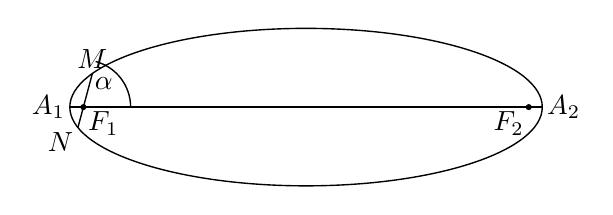
\begin{tikzpicture}[scale=1.0, line width=0.5pt,
  every node/.style={inner sep=1.5pt}]
  \draw (0,0) ellipse (3 and 1);
  \coordinate (A1) at (-3,0);
  \coordinate (A2) at (3,0);
  \coordinate (F1) at (-2.828,0);
  \coordinate (F2) at (2.828,0);
  \coordinate (M) at (-2.714,0.426);
  \coordinate (N) at (-2.897,-0.259);
  \draw (A1) -- (A2);
  \draw (M) -- (N);
  \fill (F1) circle (1.1pt);
  \fill (F2) circle (1.1pt);
  \draw (F1) ++(0.60,0) arc (0:75:0.60);
  \node[above] at (M) {$M$};
  \node[below left] at (N) {$N$};
  \node[left] at (A1) {$A_1$};
  \node[right] at (A2) {$A_2$};
  \node[below right] at (F1) {$F_1$};
  \node[below left] at (F2) {$F_2$};
  \node at (-2.57,0.30) {$\alpha$};
\end{tikzpicture}
